\section{What sets the cost of a step}
\label{sec:stepcost}

\paragraph{Step size.}
The step log confirmed the budget was applied exactly. No step scheduled more than $B$
tokens, and each run's logged prompt tokens equalled the number sent. The primary
prediction of Milestone 5 was that a step's cost tracks its scheduled tokens, measured
by the interval from one scheduling call to the next. Pooled over the seven C32
series, steps of at least 1024 tokens were followed by a median interval of 56\ms,
against 5.7\ms{} for steps of at most 64 tokens (9.8$\times$, Spearman 0.87), and the
prediction passed. At C8 the same test gave 9.0$\times$ but a Spearman correlation of
0.57, below its threshold of 0.7. Under the protocol's rule, this rejects the
hypothesis's first clause at C8.
% src: reports/milestone5-20261025T004640Z-pilot.md (predictions 1, 2); reports/milestone5p2-*-part2.md (prediction 2; Result: the pre-registered rule rejects H's first clause at C8); experiments/milestone5.md (falsification rule)

\paragraph{A lagged measure.}
The interval is confounded with the previous step. vLLM 0.29.0 can schedule step
$n{+}1$ before it processes step $n$'s results, so the interval credited to step $n$
partly reflects the cost of step $n{-}1$. The pilot found that the interval correlated
better with the previous step's tokens (0.92) than with the step's own (0.87). Some
intervals are too short to be a step's own cost: at C8 with $B{=}8192$ and $L{=}1024$,
steps of at least 1024 tokens had a median interval of 16.5\ms, while a single
1024-token chunk took a median of at least 19.5\ms{} at every context we measured
(below). At C32, prompt-carrying steps come in runs, so a lagged measure still
separates large steps from small ones, and the C32 pass is weak evidence about a
step's own cost. Part~2's execution time is tied to the step itself
(Section~\ref{sec:method}). Over the C8 block it tracked a step's own tokens better
than the interval did (Spearman 0.63 against 0.57), still below the threshold. No C32
run recorded it.
% src: reports/milestone5-*-pilot.md (Interpretation: measurement note); reports/milestone5p2-*-part2.md (C8 step-log table: len1024-budget8192-c8 16.5 ms; Part 2B table; prediction 14); vLLM 0.29.0 v1/engine/core.py (step_with_batch_queue)

\paragraph{Packing (post hoc).}
The step log also suggests why part of the tail prediction failed. At $B{=}2048$ and
$L{=}1024$, 94\% of steps carrying at least 1024 prompt tokens held two or more
prompts, and the median prompt-carrying step was a full 2048 tokens. vLLM's scheduler
fills the budget whenever prompts are waiting, so a prompt shorter than the budget
changes how often steps carry prompt work (38\% of steps at $L{=}1024$, against 77\%
at $L{=}2048$) more than how large those steps are. This fits the median falling far
(6.1 against 55\ms) while the tail fell only 19\%. Our workload favors packing: all
requests have the same lengths and start together, so they finish and return in
groups. With staggered arrivals, fewer prompts would wait at once.
% src: reports/milestone5-20261025T004640Z-pilot.md (Interpretation: short prompts are packed; step-log table)

\paragraph{Context.}
The pilot had suggested a role for context: 2048-token steps were followed by shorter
intervals at shorter prompts (45\ms{} at $L{=}1024$, 55.5\ms{} at $L{=}2048$). We
withdraw that reading. At both lengths those steps start at context 0, and the gap
follows the share of steps that carry prompt work (38\% against 77\%), as a lagged
measure would. A second pre-registered design tested context directly. We ran one
request at a time (C1) with 8192-token prompts at budgets 1024 and 2048, so every
prompt step held exactly one chunk of exactly $B$ tokens at a known context position,
and timed each chunk by its execution time (Figure~\ref{fig:context}). Chunk cost rose
almost linearly with context:
\begin{itemize}
  \item 1024-token chunks took 25.0\ms{} at context 0 and 19.5\ms{} at context
    1024, then rose to 35.9\ms{} at context 7168;
  \item 2048-token chunks rose from 41.7\ms{} at context 0 to 67.4\ms{} at context
    6144.
\end{itemize}
The deepest chunk cost 1.44$\times$ and 1.62$\times$ the first, and the Spearman
correlation between context and execution time was 0.96 in both series. From context
2048 on, each additional 1024 tokens of context added about 1.9\ms{} to a 1024-token
chunk and 3.8\ms{} to a 2048-token chunk.
% src: reports/milestone5-*-pilot.md (step-log table: 44.9 / 55.5 ms; 38% / 77%); reports/milestone5p2-20261029T000043Z-part2.md (Part 2B table; predictions 11-13; Interpretation: slopes)

These slopes match a FLOP count. A chunk of $n$ tokens at context $c$ spends about
$4ncd$ attention FLOPs per layer on the prior context, with $d{=}896$ and 24 layers.
Each 1024 tokens of context then costs 0.09 TFLOP for a 1024-token chunk and 0.18
TFLOP for a 2048-token chunk. At the tensor peak these take 1.2 and 2.4\ms; at the
40 TFLOPS that the context-0 2048-token chunk achieved, 2.3 and 4.6\ms. The measured
slopes lie between the two and double with chunk size, as the count predicts. The
first chunk of each prompt was slower than the second at $B{=}1024$ (25.0 against
19.5\ms), plausibly because of per-request setup on a request's first step; this
reading is post hoc. That setup cost lowers the ratios measured from context 0: taken
from the second chunk, the $B{=}1024$ ratio is 1.84$\times$, and at context 0 a
2048-token chunk cost 1.67$\times$ a 1024-token chunk, where FLOPs predict about
2.1$\times$.
% src: FLOP count from the model config (14 heads of 64 dimensions, 24 layers) and the A4000 datasheet; 40 TFLOPS = (1.47 linear + 0.18 attention TFLOP) / 41.7 ms; 1.84 = 35.9 / 19.5

\begin{figure}[t]
  \centering
  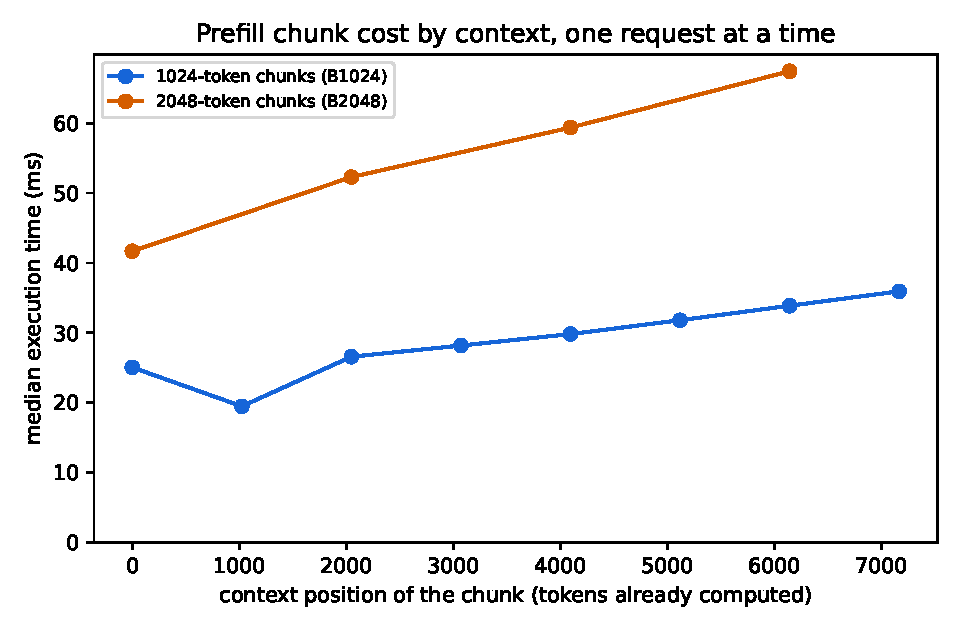
\includegraphics[width=0.55\linewidth]{milestone5-part2-context.pdf}
  \caption{Median execution time of prefill chunks by context position, one request
    at a time with 8192-token prompts (300 chunks per point).}
  \label{fig:context}
\end{figure}
